%!TEX TS-program = xelatex
%!TEX encoding = UTF-8 Unicode
% Awesome CV LaTeX Template for CV/Resume
%
% This template has been downloaded from:
% https://github.com/posquit0/Awesome-CV
%
% Author:
% Claud D. Park <posquit0.bj@gmail.com>
% http://www.posquit0.com
%
% Template license:
% CC BY-SA 4.0 (https://creativecommons.org/licenses/by-sa/4.0/)
%


%-------------------------------------------------------------------------------
% CONFIGURATIONS
%-------------------------------------------------------------------------------
% A4 paper size by default, use 'letterpaper' for US letter
\documentclass[11pt, a4paper]{awesome-cv}

% Configure page margins with geometry
\geometry{left=1.4cm, top=.8cm, right=1.4cm, bottom=1.8cm, footskip=.5cm}

% Specify the location of the included fonts
\fontdir[fonts/]

% Color for highlights
% Awesome Colors: awesome-emerald, awesome-skyblue, awesome-red, awesome-pink, awesome-orange
%                 awesome-nephritis, awesome-concrete, awesome-darknight
\colorlet{awesome}{awesome-skyblue}
% Uncomment if you would like to specify your own color
% \definecolor{awesome}{HTML}{CA63A8}

% Colors for text
% Uncomment if you would like to specify your own color
% \definecolor{darktext}{HTML}{414141}
% \definecolor{text}{HTML}{333333}
% \definecolor{graytext}{HTML}{5D5D5D}
% \definecolor{lighttext}{HTML}{999999}

% Set false if you don't want to highlight section with awesome color
\setbool{acvSectionColorHighlight}{true}

% If you would like to change the social information separator from a pipe (|) to something else
%\renewcommand{\acvHeaderSocialSep}{\quad\textbar\quad}
\renewcommand{\acvHeaderSocialSep}{\enskip\cdotp\enskip}

\usepackage{graphicx}
\usepackage{wrapfig}
\usepackage[export]{adjustbox}
\usepackage{subfigure}
\graphicspath{ {./examples/} }

%-------------------------------------------------------------------------------
%	PERSONAL INFORMATION
%	Comment any of the lines below if they are not required
%-------------------------------------------------------------------------------
% Available options: circle|rectangle,edge/noedge,left/right
\photo[noedge]{./examples/profile-Jonathan_Alves.jpg}
\name{Jonathan F.}{Alves}
\position{Business Intelligence Engineer{\enskip\cdotp\enskip}Data Expert}
\address{Estr. dos Bandeirantes, 8325 - Bloco 3, Jacarepaguá, Rio de Janeiro, 22780081, Brazil}

\mobile{(+55) 21-96407-9814}
\email{jonathan.f.alves@gmail.com}
\homepage{jalves.bi}
\github{jfalves}
\linkedin{jonathanalves}
% \gitlab{gitlab-id}
% \stackoverflow{SO-id}{SO-name}
% \twitter{@twit}
\skype{jonathan.f.alves}
% \reddit{reddit-id}
% \medium{madium-id}
% \googlescholar{googlescholar-id}{name-to-display}
%% \firstname and \lastname will be used
% \googlescholar{googlescholar-id}{}
% \extrainfo{extra informations}

\quote{``Happiness is the best measure of success."}


%-------------------------------------------------------------------------------
\begin{document}

% Print the header with above personal informations
% Give optional argument to change alignment(C: center, L: left, R: right)
\makecvheader

% Print the footer with 3 arguments(<left>, <center>, <right>)
% Leave any of these blank if they are not needed
\makecvfooter
  {\today}
  {Jonathan F. Alves~~~·~~~Curriculum Vitae}
  {\thepage}


%-------------------------------------------------------------------------------
%	CV/RESUME CONTENT
%	Each section is imported separately, open each file in turn to modify content
%-------------------------------------------------------------------------------
%-------------------------------------------------------------------------------
%	SECTION TITLE
%-------------------------------------------------------------------------------
\cvsection{Education}


%-------------------------------------------------------------------------------
%	CONTENT
%-------------------------------------------------------------------------------
\begin{cventries}

%---------------------------------------------------------
  \cventry
    {MBA. in Business Intelligence} % Degree
    {Pontifical Catholic University} % Institution
    {Rio de Janeiro, Brazil} % Location
    {Jan. 2019 - Jul. 2020} % Date(s)
    {
      \begin{cvitems} % Description(s) bullet points
        \item {Technical MBA focused on machine learning, artificial intelligence, bigdata, intelligent mathematical and statistical decision support methods.}
        % \item {\textsc{Graduation Work}: -}
        % \item {\textsc{Gpa}: -/-}
      \end{cvitems}
    }

  \cventry
    {P.Tech. in System Development and Analysis} % Degree
    {Estácio de Sá University} % Institution
    {Rio de Janeiro, Brazil} % Location
    {Jan. 2007 - Dec. 2010} % Date(s)
    {
      \begin{cvitems} % Description(s) bullet points
        \item {The course prepares professionals to create, analyze, design and implement computer information systems. It is formatted with disciplines to develop logical thinking, mastery of programming languages and project construction methodologies, etc.}
        \item {\textsc{Graduation Work}: ''\href{https://github.com/jfalves/camimsca}{Service Queue Management System Applied to Medical Clinics}''}
        \item {\textsc{Gpa}: 7.9/10}
      \end{cvitems}
    }

%---------------------------------------------------------
\end{cventries}

%-------------------------------------------------------------------------------
%	SECTION TITLE
%-------------------------------------------------------------------------------
\cvsection{Skills}


%-------------------------------------------------------------------------------
%	CONTENT
%-------------------------------------------------------------------------------
\begin{cvskills}

%---------------------------------------------------------
  \cvskill
    {ETL} % Category
    {Python, Hitachi Pentaho, Informatica Powercenter, PL/SQL} % Skills

%---------------------------------------------------------
  \cvskill
    {Databases} % Category
    {Mysql, Postgres, Oracle, Sql Server, DB2, AWS Athena, AWS Redshift, Mongodb} % Skills

%---------------------------------------------------------
  \cvskill
    {Visualization} % Category
    {Tableau, Qlik Sense/View, Power BI, Chart.io, Klipfolio} % Skills

%---------------------------------------------------------
  \cvskill
    {Analytics} % Category
    {Alteryx, RapidMiner, R} % Skills

%---------------------------------------------------------
  \cvskill
    {Certifications} % Category
    {Certified ScrumMaster\textregistered, Alteryx - Basics, Informatica Data Quality 9.0.1} % Skills
%---------------------------------------------------------
  \cvskill
    {Languages} % Category
    {Portuguese, English, Spanish} % Skills

%---------------------------------------------------------
\end{cvskills}

%-------------------------------------------------------------------------------
%	SECTION TITLE
%-------------------------------------------------------------------------------
\cvsection{Experience}


%-------------------------------------------------------------------------------
%	CONTENT
%-------------------------------------------------------------------------------
\begin{cventries}

%---------------------------------------------------------
  \cventry
    {Business Intelligence Consultant} % Job title
    {Nórdica} % Organization
    {São Paulo, Brazil} % Location
    {Mar. 2019 - Current} % Date(s)
    {
      \begin{cvitems} % Description(s) of tasks/responsibilities
        Responsible for data integration and visualization (Qlik Sense) in diverse projects, as well software migrations, from Qlik View to Qlik Sense.
      \end{cvitems}
    }

%---------------------------------------------------------
  \cventry
    {Data Engineer \& Visualization Freelancer} % Job title
    {Cognitivo.ai} % Organization
    {Remote} % Location
    {Oct. 2018 - Current} % Date(s)
    {
      \begin{cvitems} % Description(s) of tasks/responsibilities
        Working remotly on business intelligence projects, doing data integration (Python, Pentaho) and dashboards development (Tableau, Chartio).
      \end{cvitems}
    }

%---------------------------------------------------------
  \cventry
    {Bussiness Intelligence Analyst} % Job title
    {B2W Digital} % Organization
    {Rio de Janeiro, Brazil} % Location
    {Mar. 2016 - Apr. 2018} % Date(s)
    {
      \begin{cvitems} % Description(s) of tasks/responsibilities
        I have gathered requirements from stakeholders and transform them into products (Dashboards, Reports) in order to decision-making and acted as a facilitator to ensure business intelligence team flowed with no impediments, always garanting the product's quality. Also, I have done some data integration (PL/SQL, Pentaho) when needed.
      \end{cvitems}
    }

%---------------------------------------------------------
  \cventry
    {Business Intelligence Analyst \& Database Administrator} % Job title
    {Sieve} % Organization
    {Rio de Janeiro, Brazil} % Location
    {Dec. 2014 - Feb. 2016} % Date(s)
    {
      \begin{cvitems} % Description(s) of tasks/responsibilities
       I have taken care of kpi's and dashboards (Klipfolio), which provided information for business decision-making, also, supported the operational sector providing ad-hoc reports and administrated company's database (Postgresql, Mysql), performing preventive and corrective maintenance. Also, I have built a datawarehouse (Python, Pentaho) for business data centralization.
      \end{cvitems}
    }

%---------------------------------------------------------
  \cventry
    {Data Integration/Cleansing Consultant} % Job title
    {Softtek} % Organization
    {Rio de Janeiro, Brazil} % Location
    {Feb. 2010 - Nov. 2014} % Date(s)
    {
      \begin{cvitems} % Description(s) of tasks/responsibilities
        I have worked on projects for large companies, gathering requirements and developing ETL procedures (Informatica Powercenter) and data cleansing (Informatica Data Quality).
      \end{cvitems}
    }

%---------------------------------------------------------
\end{cventries}

%%-------------------------------------------------------------------------------
%	SECTION TITLE
%-------------------------------------------------------------------------------
\cvsection{Extracurricular Activity}


%-------------------------------------------------------------------------------
%	CONTENT
%-------------------------------------------------------------------------------
\begin{cventries}

%---------------------------------------------------------
  \cventry
    {Core Member} % Affiliation/role
    {B10S (B1t 0n the Security, Underground hacker team)} % Organization/group
    {S.Korea} % Location
    {Nov. 2011 - PRESENT} % Date(s)
    {
      \begin{cvitems} % Description(s) of experience/contributions/knowledge
        \item {Gained expertise in penetration testing areas, especially targeted on web application and software.}
        \item {Participated on a lot of hacking competition and won a good award.}
        \item {Held several hacking competitions non-profit, just for fun.}
      \end{cvitems}
    }

%---------------------------------------------------------
  \cventry
    {Member} % Affiliation/role
    {WiseGuys (Hacking \& Security research group)} % Organization/group
    {S.Korea} % Location
    {Jun. 2012 - PRESENT} % Date(s)
    {
      \begin{cvitems} % Description(s) of experience/contributions/knowledge
        \item {Gained expertise in hardware hacking areas from penetration testing on several devices including wireless router, smartphone, CCTV and set-top box.}
        \item {Trained wannabe hacker about hacking technique from basic to advanced and ethics for white hackers by hosting annual Hacking Camp.}
      \end{cvitems}
    }

%---------------------------------------------------------
  \cventry
    {Core Member \& President at 2013} % Affiliation/role
    {PoApper (Developers' Network of POSTECH)} % Organization/group
    {Pohang, S.Korea} % Location
    {Jun. 2010 - Jun. 2017} % Date(s)
    {
      \begin{cvitems} % Description(s) of experience/contributions/knowledge
        \item {Reformed the society focusing on software engineering and building network on and off campus.}
        \item {Proposed various marketing and network activities to raise awareness.}
      \end{cvitems}
    }

%---------------------------------------------------------
  \cventry
    {Member} % Affiliation/role
    {PLUS (Laboratory for UNIX Security in POSTECH)} % Organization/group
    {Pohang, S.Korea} % Location
    {Sep. 2010 - Oct. 2011} % Date(s)
    {
      \begin{cvitems} % Description(s) of experience/contributions/knowledge
        \item {Gained expertise in hacking \& security areas, especially about internal of operating system based on UNIX and several exploit techniques.}
        \item {Participated on several hacking competition and won a good award.}
        \item {Conducted periodic security checks on overall IT system as a member of POSTECH CERT.}
        \item {Conducted penetration testing commissioned by national agency and corporation.}
      \end{cvitems}
    }

%---------------------------------------------------------
  \cventry
    {Member} % Affiliation/role
    {MSSA (Management Strategy Club of POSTECH)} % Organization/group
    {Pohang, S.Korea} % Location
    {Sep. 2013 - Jun. 2017} % Date(s)
    {
      \begin{cvitems} % Description(s) of experience/contributions/knowledge
        \item {Gained knowledge about several business field like Management, Strategy, Financial and marketing from group study.}
        \item {Gained expertise in business strategy areas and inisght for various industry from weekly industry analysis session.}
      \end{cvitems}
    }

%---------------------------------------------------------
\end{cventries}

%%-------------------------------------------------------------------------------
%	SECTION TITLE
%-------------------------------------------------------------------------------
\cvsection{Honors \& Awards}


%-------------------------------------------------------------------------------
%	SUBSECTION TITLE
%-------------------------------------------------------------------------------
\cvsubsection{International}


%-------------------------------------------------------------------------------
%	CONTENT
%-------------------------------------------------------------------------------
\begin{cvhonors}

%---------------------------------------------------------
  \cvhonor
    {Finalist} % Award
    {DEFCON 26th CTF Hacking Competition World Final} % Event
    {Las Vegas, U.S.A} % Location
    {2018} % Date(s)

%---------------------------------------------------------
  \cvhonor
    {Finalist} % Award
    {DEFCON 25th CTF Hacking Competition World Final} % Event
    {Las Vegas, U.S.A} % Location
    {2017} % Date(s)

%---------------------------------------------------------
  \cvhonor
    {Finalist} % Award
    {DEFCON 22nd CTF Hacking Competition World Final} % Event
    {Las Vegas, U.S.A} % Location
    {2014} % Date(s)

%---------------------------------------------------------
  \cvhonor
    {Finalist} % Award
    {DEFCON 21st CTF Hacking Competition World Final} % Event
    {Las Vegas, U.S.A} % Location
    {2013} % Date(s)

%---------------------------------------------------------
  \cvhonor
    {Finalist} % Award
    {DEFCON 19th CTF Hacking Competition World Final} % Event
    {Las Vegas, U.S.A} % Location
    {2011} % Date(s)

%---------------------------------------------------------
  \cvhonor
    {6th Place} % Award
    {SECUINSIDE Hacking Competition World Final} % Event
    {Seoul, S.Korea} % Location
    {2012} % Date(s)

%---------------------------------------------------------
\end{cvhonors}


%-------------------------------------------------------------------------------
%	SUBSECTION TITLE
%-------------------------------------------------------------------------------
\cvsubsection{Domestic}


%-------------------------------------------------------------------------------
%	CONTENT
%-------------------------------------------------------------------------------
\begin{cvhonors}

%---------------------------------------------------------
  \cvhonor
    {3rd Place} % Award
    {WITHCON Hacking Competition Final} % Event
    {Seoul, S.Korea} % Location
    {2015} % Date(s)

%---------------------------------------------------------
  \cvhonor
    {Silver Prize} % Award
    {KISA HDCON Hacking Competition Final} % Event
    {Seoul, S.Korea} % Location
    {2017} % Date(s)

%---------------------------------------------------------
  \cvhonor
    {Silver Prize} % Award
    {KISA HDCON Hacking Competition Final} % Event
    {Seoul, S.Korea} % Location
    {2013} % Date(s)

%---------------------------------------------------------
  \cvhonor
    {2nd Award} % Award
    {HUST Hacking Festival} % Event
    {S.Korea} % Location
    {2013} % Date(s)

%---------------------------------------------------------
  \cvhonor
    {3rd Award} % Award
    {HUST Hacking Festival} % Event
    {S.Korea} % Location
    {2010} % Date(s)

%---------------------------------------------------------
  \cvhonor
    {3rd Award} % Award
    {Holyshield 3rd Hacking Festival} % Event
    {S.Korea} % Location
    {2012} % Date(s)

%---------------------------------------------------------
  \cvhonor
    {2nd Award} % Award
    {Holyshield 3rd Hacking Festival} % Event
    {S.Korea} % Location
    {2011} % Date(s)

%---------------------------------------------------------
  \cvhonor
    {5th Place} % Award
    {PADOCON Hacking Competition Final} % Event
    {Seoul, S.Korea} % Location
    {2011} % Date(s)

%---------------------------------------------------------
\end{cvhonors}

\pagebreak
  %-------------------------------------------------------------------------------
  %	SECTION TITLE
  %-------------------------------------------------------------------------------
  \cvsection{Projects}


  %-------------------------------------------------------------------------------
  %	CONTENT
  %-------------------------------------------------------------------------------
  \cvsubsection{Project\#1}

  %---------------------------------------------------------
    \cvparagraph
    {
      \begin{wrapfigure}{r}{0.5\textwidth}
        \centering
        \vspace{-10pt}
        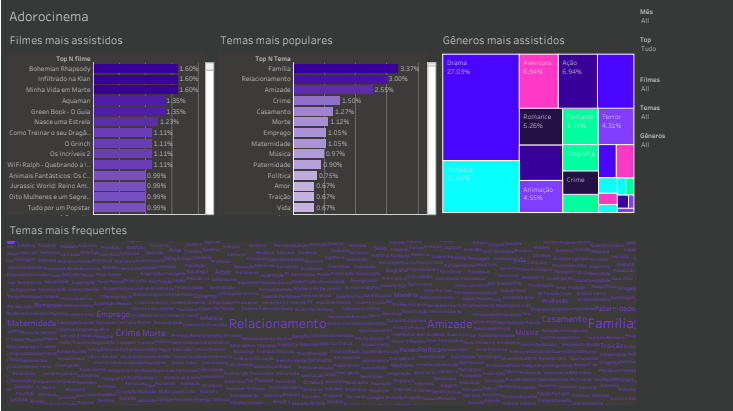
\includegraphics[width=0.5\textwidth]{project1}
      \end{wrapfigure}
      A marketing and advertising company needed dashboards to track social networking data, which was enriched by its employees by adding keywords using Google sheets.

      When I started the project, my role was to create database model and dashboards but there was legacy python code from which I made improvements by adding a database management framework (ORM). Later, there was a need of database migration, confirming the right decision to add an ORM.

      \textsc{Techonologies used}: Python, SQL Alchemy, SQL Server, Postgres, Api Google Docs, Tableau.
      \vfill
    }

  %---------------------------------------------------------

  \cvsubsection{Project\#2}

   %---------------------------------------------------------
    \cvparagraph
    {
      \begin{wrapfigure}{r}{0.5\textwidth}
        \centering
        \vspace{-10pt}
        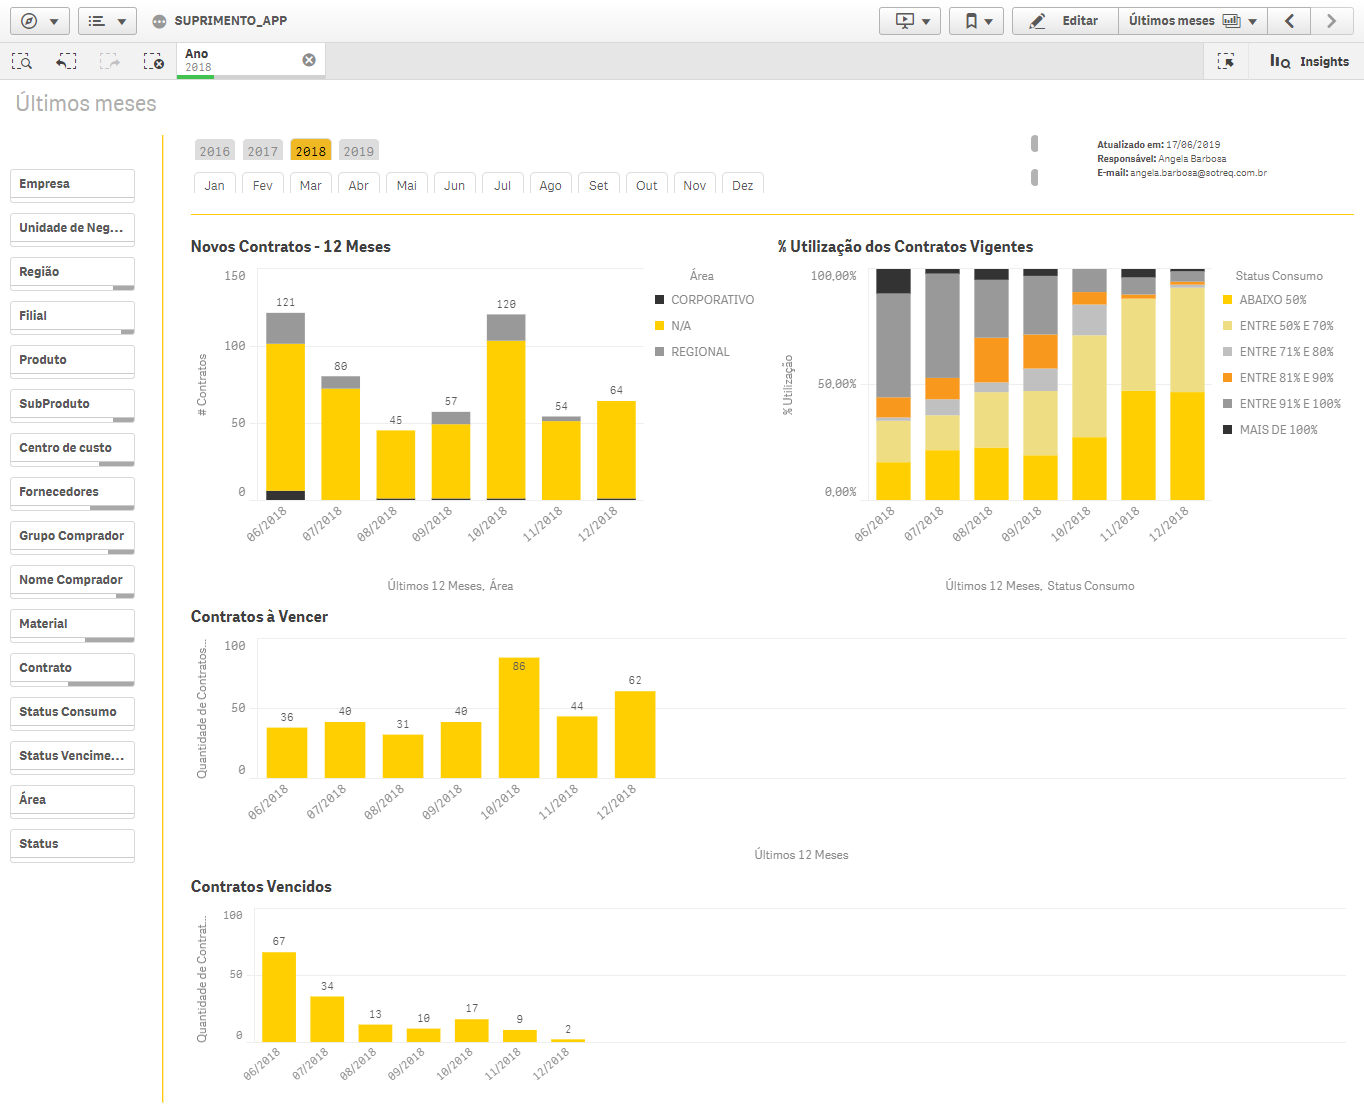
\includegraphics[width=0.5\textwidth]{project2}
      \end{wrapfigure}
      An engineering machinery company kept all of its supplier's contract data in the SAP system, it must somehow audit these contracts.

      Data was extracted from SAP using Qlik View's own language and a special connector provided by the software. These data were modeled and presented in the Qlik Sense tool.

      \textsc{Techonologies used}: Qlik View, Qlik Sense.
      \vfill
    }

   %---------------------------------------------------------

    \cvsubsection{Project\#3}

    %---------------------------------------------------------
     \cvparagraph
     {
      \begin{wrapfigure}{r}{0.5\textwidth}
        \centering
        \vspace{-10pt}
        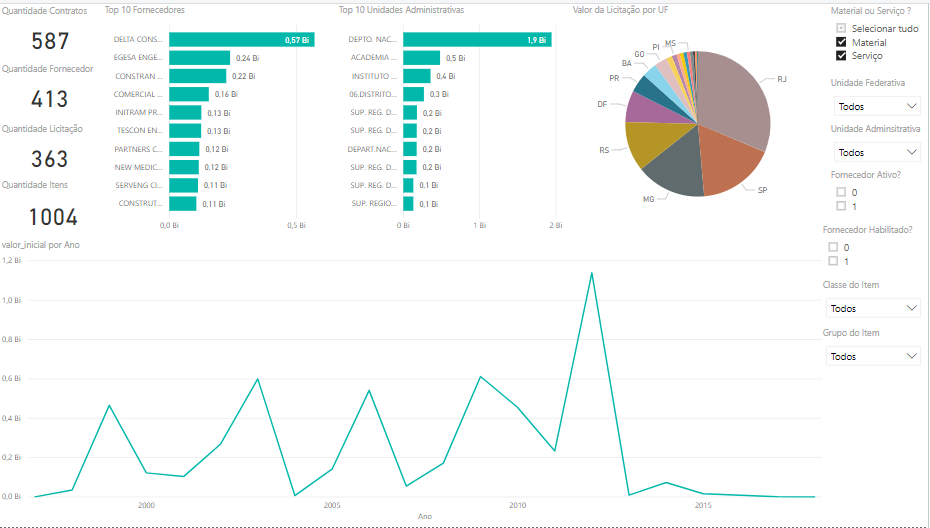
\includegraphics[width=0.5\textwidth]{project3}
      \end{wrapfigure}
      This was one of my projects for the MBA in Business Intelligence, where I compiled public procurement data from Brazilian government.

      The data was consumed through a web API, generating flat files. These files were inserted into database and made available by a visualization tool.

      Over time I have intention to make this vision available to the Brazilian population.

      \textsc{Techonologies used}: Pentaho, Postgres, Power BI
      \vfill
    }
   %---------------------------------------------------------

%%-------------------------------------------------------------------------------
%	SECTION TITLE
%-------------------------------------------------------------------------------
\cvsection{Writing}


%-------------------------------------------------------------------------------
%	CONTENT
%-------------------------------------------------------------------------------
\begin{cventries}

%---------------------------------------------------------
  \cventry
    {Founder \& Writer} % Role
    {A Guide for Developers in Start-up} % Title
    {Facebook Page} % Location
    {Jan. 2015 - PRESENT} % Date(s)
    {
      \begin{cvitems} % Description(s)
        \item {Drafted daily news for developers in Korea about IT technologies, issues about start-up.}
      \end{cvitems}
    }

%---------------------------------------------------------
  \cventry
    {Undergraduate Student Reporter} % Role
    {AhnLab} % Title
    {S.Korea} % Location
    {Oct. 2012 - Jul. 2013} % Date(s)
    {
      \begin{cvitems} % Description(s)
        \item {Drafted reports about IT trends and Security issues on AhnLab Company magazine.}
      \end{cvitems}
    }

%---------------------------------------------------------
\end{cventries}

%%-------------------------------------------------------------------------------
%	SECTION TITLE
%-------------------------------------------------------------------------------
\cvsection{Program Committees}


%-------------------------------------------------------------------------------
%	CONTENT
%-------------------------------------------------------------------------------
\begin{cvhonors}

%---------------------------------------------------------
  \cvhonor
    {Problem Writer} % Position
    {2016 CODEGATE Hacking Competition World Final} % Committee
    {S.Korea} % Location
    {2016} % Date(s)

%---------------------------------------------------------
  \cvhonor
    {Organizer \& Co-director} % Position
    {1st POSTECH Hackathon} % Committee
    {S.Korea} % Location
    {2013} % Date(s)

%---------------------------------------------------------
  \cvhonor
    {Staff} % Position
    {7th Hacking Camp} % Committee
    {S.Korea} % Location
    {2012} % Date(s)

%---------------------------------------------------------
  \cvhonor
    {Problem Writer} % Position
    {1st Hoseo University Teenager Hacking Competition} % Committee
    {S.Korea} % Location
    {2012} % Date(s)

%---------------------------------------------------------
  \cvhonor
    {Staff \& Problem Writer} % Position
    {JFF(Just for Fun) Hacking Competition} % Committee
    {S.Korea} % Location
    {2012} % Date(s)

%---------------------------------------------------------
\end{cvhonors}



%-------------------------------------------------------------------------------
\end{document}
